
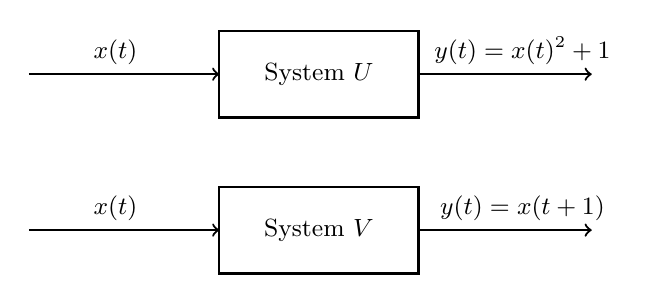
\begin{tikzpicture}[scale=1.1, every node/.style={font=\small}]

    % System U block and arrows
    \draw[thick] (0,1.8) -- (1.5,1.8);
    \draw[thick, ->] (1.5,1.8) -- (2.2,1.8);
    \node[above] at (1.0,1.8) {$x(t)$};

    \draw[thick] (2.2,1.3) rectangle (4.5,2.3);
    \node at (3.35,1.8) {System $U$};

    \draw[thick, ->] (4.5,1.8) -- (6.5,1.8);
    \node[above] at (5.7,1.8) {$y(t) = x(t)^2 + 1$};

    % System V block and arrows
    \draw[thick] (0,0) -- (1.5,0);
    \draw[thick, ->] (1.5,0) -- (2.2,0);
    \node[above] at (1.0,0) {$x(t)$};

    \draw[thick] (2.2,-0.5) rectangle (4.5,0.5);
    \node at (3.35,0) {System $V$};

    \draw[thick, ->] (4.5,0) -- (6.5,0);
    \node[above] at (5.7,0) {$y(t) = x(t + 1)$};

\end{tikzpicture}
